\beginsong{Uno - Due - Tre}[
    wuw={Kilian Hähn, Jakob Hoffmann}, 
    jahr={2017},
    lager={VCP Bundeslager 2017 \emph{''Weitblick''}, hessisches Teillager \emph{''Villa Resistenza''}},
    ]

\beginchorus
\emph{\[C]Uno, Due, \[G]Tre} - dich im \[C]Kreis,  
\emph{Quattro, Cinque, \[G]Sei} - da\[C]bei,
\emph{Sette, Otto, \[G]Nove} - \[F]schön. 
\emph{Di\[F]eci} - macht am \[G]Ende \[C]zehn.
\endchorus

\beginverse
Das \[Am]Problem mit den Nächten ist der \[G]Morgen danach,
du bist \emph{\[Am]tutti completi}, \[E]durch und verstrahlt.
\emph{Il pro\[C]fumo}, \emph{di caffè} und die \emph{\[G]sole} im Zelt
macht es \[E]uns etwas leichter, doch was \[Am]hilft und was \[G]zählt, ist ...
\endverse

\printchorus

\beginverse
Das Pro^blem mit dem Essen, jeder ^weiß es genau,
es ist ^stets falsch bemessen und nicht ^heiß sondern lau.
Mach' die \emph{^pasta al dente}, lass' den ^Zimt nicht im Tschai
Gönn' dir ^auch mal \emph{gelato}. Wie viel ^Kugeln? Eine? Zwei? ^Drei? 
\endverse

\printchorus

\beginverse
Das Pro^blem mit der Liebe, mit \emph{ti ^amo} und so, 
das sind ^erstmal die Triebe und das ^Partnerniveau.
Und wie s^oll man's beginnen, man wird \emph{^rosso} und stumm
aber ^alles auf einmal ist \emph{stu^pido} - da^rum...
\endverse

\printchorus

\beginverse
Das Pro^blem mit der Welt: Sie ist ^groß und bewohnt
von ein ^paar \emph{Grande stronzi} die ge^hören entthront.
In der \emph{^Villa Resistenza} fangen ^wir schonmal an 
mit viel ^Schwung und \emph{pazienza} zählt was ^jeder so ^kann...
\endverse

\repchorus{2}

% \beginverse
% Das Pro^blem mit dem Wetter ist hin^länglich bekannt,
% man be^kommt nasse Füße oder ^hat Sonnenbrand.
% Doch die \emph{^Quattro Stagioni} sind nun^mal so gestrickt,
% nach der ^Sonne kommt Regen eben ^\emph{mezzo} ge^mixt.
% \endverse

% \repchorus{2}


\endsong

\begin{intersong}
\ifthenelse{\boolean{pics}}{
	\vfill
	\centering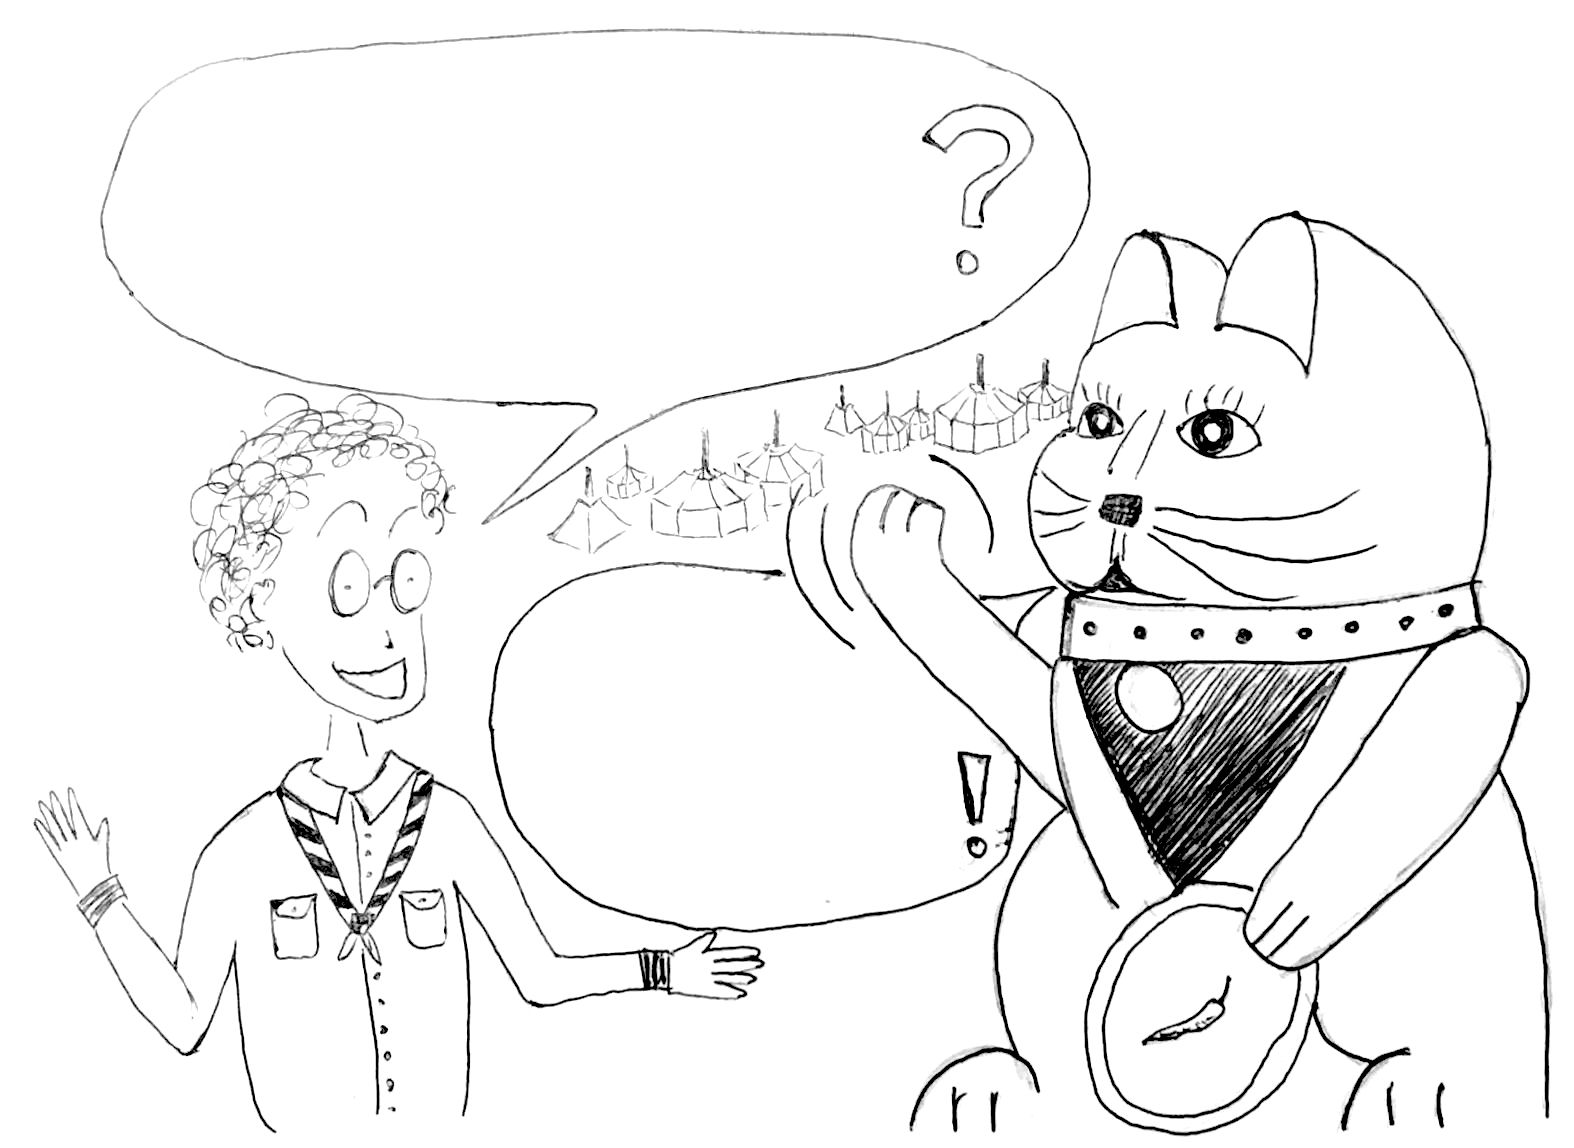
\includegraphics[width=\textwidth]{Bilder/Katzo.jpg}
}{}
\end{intersong}